\chapter{Optimal Control and Dynamic Programming}
% TODO: need to improve the flow of this section
% - decide on order of presentation for different concepts; deterministic vs stochastic, perfect vs imperfect state information, continuous vs discrete time


In this section we will introduce the fundamental concepts of optimal control in discrete and continuous time. In particular, we introduce the principle of optimality, which enables dynamic programming. Dynamic programming allows us to solve optimal control problems by recursively solving sub-problems, and this approach is (arguably) the most important concept in our study of optimal control. In addition to studying dynamic programming and the principle of optimality in discrete and continuous time for both deterministic and stochastic systems, we will introduce optimal control algorithms for discrete state spaces.

\section{The Optimal Control Problem}

\subsection{Optimal Control in Continuous Time}

We will first outline the \textit{deterministic}, \textit{continuous-time} optimal control problem that we will aim to solve, before moving on to alternative problem statements including stochasticity and discrete-time. We will denote the state at time $t$ as $\st(t) \in \R^n$, and the control as $\ac(t) \in \R^m$. We will also occasionally write these as $\st_t$ and $\ac_t$, respectively. We will write the continuous-time systems dynamics as 
\begin{equation}
    \stdot(t) = \bm{\f}(\st(t),\ac(t),t).
    \label{eq:2_ct_dyn}
\end{equation}
We will refer to a history of control input values during an interval $[t_0,t_f]$ as a control history, and we will refer to a history of state values over this interval as a state trajectory. 

Different control problems may call for various constraints. For example, we may constrain a quadrotor to only fly in space not occupied by obstacles. Examples of constraints we will see are
\begin{itemize}
    \item Initial and final conditions, $\st(t_0) = \st_0$, $\st(t_f) = \st_f$
    \item Trajectory constraints, $\munderbar{\st} \leq \st(t) \leq \bar{\st}$
    \item Control limits, $\munderbar{\ac} \leq \ac(t) \leq \bar{\ac}$.
\end{itemize}
A state trajectory and control history that satisfy the constraints during the entire time interval $[t_0,t_f]$ are called admissible trajectories and admissible controls, respectively. 

Finally, we will define the performance measure, 
\begin{equation}
    J = \cost_f(\st(t_f),t_f) + \int_{t_0}^{t_f} \cost(\st(t),\ac(t),t) dt
    \label{eq:2_perf}
\end{equation}
where $\cost$ is the instantaneous cost function, and $\cost_f$ is the terminal state cost. We are now able to state the continuous-time optimal control problem. 
We aim to find an admissible control, $\ac^*$, which causes the system (\ref{eq:2_ct_dyn}) to follow an admissible trajectory, $\st^*$, that minimizes the performance measure given by (\ref{eq:2_perf}). The minimizer $(\st^*,\ac^*)$ is called an optimal trajectory-control pair. 

% write as optimization problem

Note, first of all, that this is an extremely general problem formulation. We have not fixed our system dynamics, cost function, or specific constraints. We can't, in general, guarantee the existence or uniqueness of the optimal solution. 

There are two possible solution forms for the optimal control. The first, $\ac^* = e(\st(t_0),t)$ is referred to as an open-loop solution. This is an input function that is applied to the system, without using feedback. Practically, such solutions usually require augmentation with a feedback controller, as small model mismatch may lead to compounding errors. The second possible solution form is a feedback policy, $\ac^* = \pol(\st(t),t)$. This feedback law maps all state-time pairs to an action and thus is usually more robust to possible model mismatch. However, depending on the particular problem formulation, open-loop solutions may be easier to compute. 
% add discussion of discrete time optimal control problem?

\subsection{Optimal Control in Discrete Time}

In the previous section, we have developed an optimal control problem statement in continuous time. This approach to system modeling is likely familiar to readers coming from a background in the physical sciences; in particular, physical models from mechanical and electrical engineering will often be stated as differential equations, and so a problem formulation in continuous time is natural. Readers from backgrounds in computer science or operations research on the other hand may be more familiar with dynamics expressed as discrete time difference equations. Moreover, such an approach is more natural for implementation on a digital computer, and thus fluency mapping between these two settings is an important skill. Finally, while work in the optimal control literature discusses both the continuous and discrete time case, the literature in reinforcement learning and artificial intelligence typically presents problems in discrete time.

We will index time with $k$, where one increment of this index is equal to some increment of time $\Delta t$. Thus, $\st_k = \st(k \Delta t)$. We will write $N$ for the final time. Then, we will write our system dynamics as 
\begin{equation}
    \st_{k+1} = \bm{\f}_k(\st_k, \ac_k)
\end{equation}
and our performance measure as 
\begin{equation}
    \J = \cost_N(\st_N) + \sum_{k=0}^{N-1} \cost(\st_k, \ac_k, k)
\end{equation}
where $\cost$ is now a stage-wise cost function, $\cost_N$ is a terminal cost function, and the integral of the continuous time formulation is replaced with a sum. 

% TODO need to introduce stochastic optimal control problem

\subsection{Markovian Decision Problems}

Before moving to the principle of optimality, we will formalize the setting in which we will operate for the duration of this class. In particular, we will outline \textit{Markovian} decision problems, variations in their presentation, as well as extensions of this framework. We will first discuss the \textit{perfect state information} case, in which the system state summarizes the full history of the system. We will then briefly discuss the \textit{imperfect state information} case. Typically, finding optimal solutions in this case is much harder than in the perfect state information case. We will introduce the incomplete state information setting only briefly, and in the next chapter we will discuss one practical case in which the imperfect case can be solved effectively. 

\subsubsection{MDPs}

We present the Markov decision process in discrete time, and the continuous time case will looks similar. The fundamental idea behind Markov Decision Processes (MDPs) is that the state dynamics are \textit{Markovian}, or obey the \textit{Markov property}. This property says that all information about the previous history of the system is summarized by its current state. While we have so far considered deterministic dynamics, we will consider probabilistic dynamics of the form 
\begin{equation}
    \st_{k+1} = \bm{\f}_k(\st_k, \ac_k, \w_k)
\end{equation}
where $\w_k$ is a stochastic disturbance, with $\w_j$ independent of $\w_i$ for $i \neq j$. This noise term at time $k$ may depend on the state and action at time $k$, but it is independent of the state and action at other time steps. This noise is typically referred to as the \textit{process noise}. Given this probabilistic dynamics model, we can reason about our conditional distribution of $\st_{k+1}$ given our current state $\st_k$ and action $\ac_k$, which we will write $p(\st_{k+1} \mid \st_k, \ac_k)$. Let 
\begin{equation}
\bm{h}_k =(\st_0, \ac_0, \cost_0, \ldots, \st_k, \ac_k)    
\end{equation} 
where $\cost_i$ is the accrued cost at timestep $i$. Then, a system is said to be Markovian if
\begin{equation}
    p(\st_{k+1} \mid \st_k, \ac_k) = p(\st_{k+1} \mid \bm{h}_k).
\end{equation}
% TODO make this a formal definition

In addition to Markovian dynamics, we require an \textit{additive} cost function, $\cost(\st_k, \ac_k, k)$. Finally, we will define the state space $\mathcal{X}$ and action space $\mathcal{U}$, such that $\st_k \in \mathcal{X}$, $\ac_k \in \mathcal{U}$ for all $k$. Given these ingredients, we will define the Markov decision process as the tuple $(\mathcal{X}, \mathcal{U}, \bm{\f}, \cost)$. 
% TODO define additive cost function
% TODO formal MDP def

Are these ingredients sufficient to completely define the optimal control problem introduced in the last section? Or equivalently, given the elements of this tuple, can we specify everything about an optimal control problem? The answer is no: we have not included the constraints (for example, control constraints), the final time, or the initial state. Are these elements necessary for the specification of an optimal control problem? We will break these elements down individually.

\paragraph{Constraints.} The control literature frequently includes constraints in the optimal control problem setting. For example, control limits are necessary to ensure commanded actions are physically realizable. In contrast, the artificial intelligence community typically does not consider constraints. For deterministic dynamics, we can include constraints in the cost function: if a constraint is violated, a cost of $\infty$ is returned. Such an approach is common in the literature on optimization \cite{boyd2004convex}. However, this leads to a problem in the stochastic case. Imagine some deterministic dynamics with an additive Gaussian noise term. If we impose state constraints on this system, the infinite support of the Gaussian noise will lead to a non-zero probability of constraints violation at every time step. The tension between stochastic dynamics and constraints is resolved in part by the constrained MDP formulation \cite{altman1999constrained}, in which a budget on constraint violation is allowed. The objective, then, is satisfying the constraint violation budget while minimizing the cost. Generally, however, designing meaningful constraints with stochastic dynamics is an active research problem in the control community. 
% add references

\paragraph{Final time.} A final time may be desired by a system designer, and thus they may choose to include this in their optimal control problem. But, is it necessary to include? Imagine an infinite-horizon optimal control problem, in which we plan a feedback policy that will execute for all time. If there exists a state that the system can reach with finite cost, for which the cost for the rest of the problem is finite (for example, a state for which we can achieve zero cost for the rest of time), then the total cost will be finite. If this is not satisfied, then the total cost is infinite. This is problematic, as it removes the ability to distinguish between different control policies, as both will receive the same (infinite) total cost. This can be resolved in several ways. As discussed in the previous section, we can limit the problem setting to a finite final time. In the infinite horizon case, we could also scale the cost accrued at each timestep so that the total cost is finite. One approach is discounting, in which cost is scaled by a time-varying term. An alternative (but less common) approach is to consider \textit{average} cost, as opposed to total cost. 


\paragraph{Initial State.} In the optimal control problem defined previously, we assumed knowledge of the initial state. This knowledge is important if we are designing an \textit{open-loop} sequence of controls. If we are searching for an optimal \textit{control policy}, we do not require the initial state, as we will find a policy that is optimal for all states. The difference between these two approaches will be discussed in depth later in this section. In reinforcement learning where you assume episodic interaction with a system, it is typical to assume a known initial state or a distribution over initial states. This is important as these algorithms typically result in sub-optimal control policies that perform better close to the regions of the state space where they have observed data, and perform worse further from their previous experience. 

\subsection{Optimal Control with Incomplete State Information}

In the definition of the Markov decision process, we assumed two necessary features of the dynamics. First, we assumed the dynamics were Markovian; the state contained all information about the history of the system. Second, we assumed that we could directly observe the state of the system (the \textit{perfect information} assumption. 
We now consider the case in which direct, perfect state information isn't available, which we refer to as the \textit{imperfect state information} setting. We have noise-corrupted measurements
\begin{align}
    \ob_{k} &= \bm{\h}_k(\st_k, \wob_{k}), \,\, k=0,\ldots,N-1
\end{align}
where $\wob_k$ is a noise term which we refer to as the \textit{measurement noise}. This measurement noise is characterized by distribution 
\begin{equation}
    p(\cdot\mid \st_k,\ldots,\st_0,\ac_{k-1},\ldots,\ac_0,\w_{k-1},\ldots,\w_{0},\wob_{k-1},\ldots,\wob_{0})
\end{equation}
and the initial state $\st_0$ is distributed according to $p(\st_0)$. We will define the information vector as
\begin{equation}
    \I_k = [\ob_0^T, \ldots, \ob_k^T, \ac_0^T, \ldots, \ac_{k-1}^T]^T.
\end{equation}
Armed with this, we will consider \textit{admissible} policies $\pi(\I_k) \in \mathcal{U}_k$, which implies they are \textit{causal} --- they do not rely on information only available in the future. The goal of the control problem, then is to minimize 
\begin{equation}
    \E_{\st_{0},\w_{0:N-1},\wob_{0:N-1}} \left[ \cost_T(\st_N) + \sum_{k=0}^{N-1} \cost(\st_k, \pol(\I_k),\w_{k}) \right].
\end{equation}
Treating this problem as a perfect state information problem and attempting to solve directly results in several problems. In addition to the standard difficulties associated with applying DP to generic problems, $\I_k$ has expanding dimension over the length of the problem. Alternatively, we may reason in terms of sufficient statistics: quantities that summarize all of the informational content of $\I_k$. For example, if we can construct a conditional distribution over state, $p(\st_k\mid\I_k)$, we can design a policy of the form $\pol_k(p(\st_k\mid\I_k))$. However, such an approach is typically only tractable in a very limited group of settings. We will discuss one such setting where this approach is tractable in the next chapter, when we discuss the \textit{linear quadratic Gaussian} control setting; we will expand on the general difficulty of optimal control with incomplete state information in the second half of this text. Analogously to the definition of the MDP, we refer to an MDP augmented with an observation function $\h(\cdot,\cdot)$ as a partially-observed MDP (POMDP). 

\section{Dynamic Programming and the Principle of Optimality}

\begin{figure}[t]
    \centering
    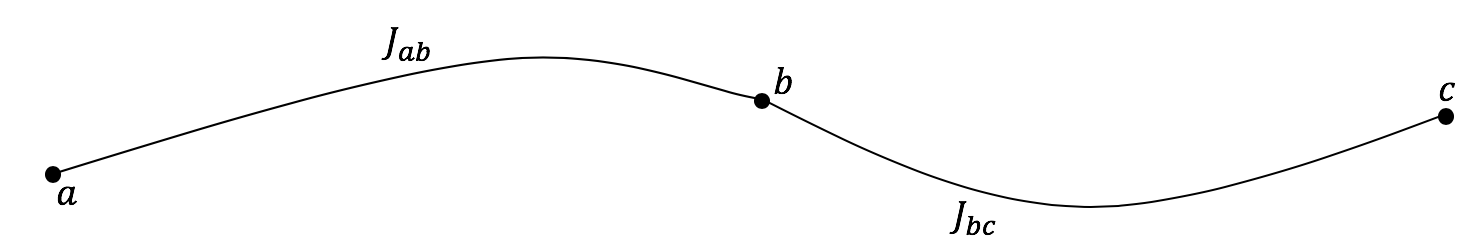
\includegraphics[width=0.8\linewidth]{figs/optimality.png}
    \caption{An optimal trajectory connecting point $a$ to point $c$. There are no better (lower cost) trajectories than the sub-trajectory connecting $b$ and $c$, by the principle of optimality.}
    \label{fig:opt1}
\end{figure}

We will now outline the principle of optimality, and the method of dynamic programming (DP), one of two main approaches to solving the optimal control problem. The second, so-called variational approaches based on Pontryagin's Maximum Principle (PMP) will be discussed in future chapters. While dynamic programming has the strong advantage compared to variational methods of yielding a feedback policy, exactly solving the dynamic programming problem is infeasible for many systems. We will address special cases in which the DP problem can be solved exactly, and approximate methods that work for a wide variety of systems. In particular, in this chapter we will discuss exhaustive approaches to dynamic programming for discrete state space problems; such methods may be used as an approximation method for continuous state space problems. In the next chapter we discuss a special case in which dynamic programming is tractable for continuous state spaces. Again, this special case is used for useful approximations for intractable problems. 
We will first introduce DP for discrete time systems, before extending these methods to the continuous time setting in the next section.

\subsection{Dynamic Programming and the Principle of Optimality}

The principle of optimality is as follows. Figure \ref{fig:opt1} shows a trajectory from point $a$ to $c$. If the cost of the trajectory, $J_{ac} = J_{ab} + J_{bc}$, is minimal, then $J_{bc}$ is also a minimum cost trajectory connecting $b$ and $c$. The proof of this principle, stated informally, is simple. Assume there exists an alternative trajectory connecting $b$ and $c$, for which we will write the cost as $\tilde{J}_{bc}$, that achieves $\tilde{J}_{bc} < J_{bc}$. Then, we have 
\begin{align}
    \tilde{J}_{ac} &= J_{ab} + \tilde{J}_{bc}\\
    &< J_{ab} + J_{bc}\\
    &= J_{ac},
\end{align}
and thus $J_{ac}$ isn't minimal. More formally,

\begin{theorem}[Discrete-time Principle of Optimality: Deterministic Case]
Let $\pi^* = (\pi_0^*, \ldots, \pi^*_{N-1})$ be an optimal policy. Assume state $\st_k$ is reachable. Consider the subproblem whereby we are at $\st_k$ at time $k$ and we wish to minimize the cost-to-go from time $k$ to time $N$. Then the truncated policy $(\pi_k^*, \ldots, \pi^*_{N-1})$ is optimal for the subproblem.
\end{theorem}

Dynamic programming, intuitively, proceeds backwards in time, first solving simpler shorter horizon problems. If we have found the optimal policy for times $k+1$ to $N-1$, along with the associated cost-to-go for each state, choosing the optimal policy for time $k$ is a one step optimization problem. More concretely, dynamic programming iterates backward in time, from $N-1$ to $0$, with
\begin{align}
    \J_N(\st_N) &= \cost_N(\st_N)\\
    \J_k(\st_k) &= \min_{\ac_k \in \mathcal{U}(\st_k)} \left\{ \cost_k(\st_k,\ac_k,k) + \J_{k+1}(\f(\st_k,\ac_k,k)) \right\}.
    \label{eq:DP_rec}
\end{align}
Note that here we have considered only deterministic dynamical systems (there is no stochastic disturbance). Equation (\ref{eq:DP_rec}) is one form of the \textit{Bellman equation}, one of the most important relations in optimal control. Critically, this approach changes the optimization problem associated with the optimal control problem from one in which optimization is performed over a sequence of actions of length $N$, to a collection of $N$ one step optimization problems. 

Dynamic programming raises many practical issues if one were to attempt to apply it directly in general. To perform the recursion, $\J_{k+1}$ must be known for all $\st_{k+1}$ (or more precisely, all $\st_{k+1}$ that are reachable from $\st_k$). If the state space is discrete (and relatively small), this is tractable as the cost-to-go may just be maintained in tabular form. We will address this case later in this section. However, for general systems, we can not expect to be able to compute the cost-to-go for all states. Possible approaches to make the DP approach tractable are discretizing the state space, approximating the cost-to-go (i.e. restricting the family of functions that $\J_{k+1}$ may be in), or interpolating between cost-to-go computed for a finite set of states. 

% should talk about the limitations of each of these methods

% should talk about how this yields a globally optimal, closed-loop policy

% add discrete DP example 


\subsection{Generalizing the Principle of Optimality: Stochastic Case}

% move this to stochastic control intro
We consider systems of the form
\begin{equation}
    \st_{k+1} = \f_k(\st_k,\ac_k,\w_k), \,\, k=0,\ldots,N-1
\end{equation}
where $\w_k \sim p(\cdot \mid \st_k, \ac_k)$ is the disturbance or noise. We write the expected cost under policy $\pol = \{\pol_0, \ldots, \pol_{N-1}\}$ as
\begin{equation}
    \label{eq:stoch_bellman}
    \J^\pi(\st_0) = \E_{\w_{0:N-1}} \left[ \cost_N(\st_N) + \sum_{k=0}^{N-1} \cost_k(\st_k,\pol_k(\st_k),\w_k) \right].
\end{equation}
Then, the stochastic control problem we wish to solve is to find
\begin{equation}
    \J^*(\st_0) = \min_\pol \J^\pol(\st_0).
\end{equation}
In contrast to the deterministic optimal control problem, we are specifically interested in finding the optimal closed-loop \textit{policy} in the stochastic case. Closed-loop policies can achieve lower cost than open-loop action sequences when disturbances are present, as they take advantage of current state information in their action selection. Thus, if disturbances cause a system to leave the nominal open-loop trajectory, a policy will continue to act optimally from that new state, whereas an open-loop sequence of actions will potentially act sub-optimally. 
% Finally, we have assumed we are operating in a \textit{risk-neutral} setting. This risk neutrality corresponds to the expectation in (\ref{eq:stoch_bellman}), which could be replaced by any \textit{risk metric}, which maps a distribution over outcomes to a scalar.
% expand on risk sensitive stochastic optimal control


We can now state the principle of optimality for the stochastic optimal control problem. Note that this is a strict generalization of the deterministic case. 

\begin{theorem}[Discrete-time Principle of Optimality: Stochastic Case]
Let $\pi^* = (\pi_0^*, \ldots, \pi^*_{N-1})$ be an optimal policy. Assume state $\st_k$ is reachable. Consider the tail subproblem
\begin{equation}
\E_{w_{i:N-1}}\left[ \cost_T(\st_N) + \sum_{k=i}^{N-1} \cost_k(\st_k,\pol_k(\st_k),\w_k) \right].
\end{equation}
Then the truncated policy $(\pi_i^*, \ldots, \pi^*_{N-1})$ is optimal for the subproblem.
\end{theorem}
The intuition behind the stochastic principle of optimality is effectively the same as for the deterministic, and the proof is also based on decomposition of the total cost into two cost terms. This is possible due to the linearity of expectation. Stated simply, if a better policy existed for the tail problem, this would imply $\pol^*$ is suboptimal. 

The stochastic version of the principle of optimality leads to a concomitant dynamic programming algorithm, which takes the form
\begin{align}
    \J_N(\st_N) &= \cost_N(\st_N)\\
    \J_k(\st_k) &= \min_{\ac_k \in \mathcal{U}(\st_k)} \E_{w_k} \left[ \cost_k(\st_k,\ac_k,\w_k) + \J_{k+1}(\f(\st_k,\ac_k,\w_k)) \right]
    \label{eq:DP_rec_stoch}
\end{align}
and the optimal policy is
\begin{align}
    \pol^*_k(\st_k) &= \argmin_{\ac_k \in \mathcal{U}(\st_k)} \E_{w_k} \left[ \cost_k(\st_k,\ac_k,\w_k) + \J_{k+1}(\f(\st_k,\ac_k,\w_k)) \right].
    \label{eq:DP_rec_stoch}
\end{align}


\section{Optimal Control in Discrete State Spaces}

We will now look at practical algorithms that use dynamic programming. The problem setting we consider for these methods are \textit{discrete state space} and \textit{discrete action space} methods. We will first discuss \textit{policy evaluation}: given some policy $\pi$ and MDP $\mathcal{M}$, we aim to determine the associated expected total cost (or value function), $\J_{\pol}$. In this section we will assume a deterministic policy, but this assumption is easily relaxed.

\subsubsection{Policy Evaluation}

The total expected cost associated with a state $\ac$ may be written as 
\begin{equation}
    \J_k^{\pol}(\st) \gets \cost_k(\st, \pol(\st)) + \sum_{\st' \in \statespace} p(\st' \mid \st, \pol(\st)) J^{\pol}_{k+1}(\st'). 
\end{equation}
Given a model of the dynamics, which we (for now) will assume known, we exactly have access to the density $p(\st' \mid \st, \pol(\st))$. Thus, the algorithm proceeds backward in time, exactly computing this expectation each time. 

While this is intuitive for the finite horizon setting, what about the infinite horizon problem setting? This same backward iteration can be repeated until convergence. It will, in the limit, converge to the true value function. Note that for infinite horizon problems, the value function is not time varying.
% TODO add more on this
% TODO add algorithm block

\subsubsection{Value Iteration}

Having discussed the computation of the value function for a fixed policy, we now proceed to the policy improvement setting, in which we aim to compute the optimal policy. \textit{Value iteration} follows closely from the policy evaluation setting. In particular, for each $\st \in \statespace$, we perform
\begin{equation}
    \J^*_k(\st) \gets \min_{\ac \in \actionspace} \left\{\cost_k(\st, \ac) + \sum_{\st' \in \statespace} p(\st' \mid \st, \ac) J^*_{k+1}(\st') \right\}. \label{eq:value_itr}
\end{equation}
This process is iterated backward in time, for all states following the dynamic programming process. This yields the optimal value function, but has not given us the optimal policy. This may be computed via 
\begin{equation}
    \pol^*_k(\st) \gets \argmin_{\ac \in \actionspace} \left\{\cost_k(\st, \ac) + \sum_{\st' \in \statespace} p(\st' \mid \st, \ac) J^*_{k+1}(\st') \right\}. 
\end{equation}
Thus while performing value iteration, we store only the value function. Given this, we can extract the policy from a one step optimization problem. 

As a useful tool that will appear throughout our discussion of reinforcement learning in particular, we will define the state-action value function (or Q function as it is more typically called) as 
\begin{equation}
    Q^{\pol}_k(\st, \ac) = \cost_k(\st, \ac) + \sum_{\st' \in \statespace} p(\st' \mid \st, \ac) J^{\pol}_{k+1}(\st').
\end{equation}
This represents the total expected cost associated with taking action $\ac$, followed by acting according to policy $\pol$ for the remainder of the problem. The Q function is extremely useful because of how it relates to the previously introduced quantities that appear throughout this section. First, note that 
\begin{equation}
    \J^\pol_k(\st) = Q^{\pol}_k(\st, \pol(\st))
\end{equation}
and 
\begin{equation}
    \J^*_k(\st) = \min_{\ac \in \actionspace} Q^{*}_k(\st, \ac).
\end{equation}
Note also that 
\begin{equation}
    \pol^*_k(s) = \argmin_{\ac \in \actionspace} Q^{*}_k(\st, \ac).
\end{equation}
A similar approach to value iteration may be performed using the Q function. Note that \eqref{eq:value_itr} is equivalent to 
\begin{equation}
    \J^*_k(\st) \gets \min_{\ac \in \actionspace} Q^*_k(\st, \ac)
\end{equation}
and thus we can iterate backward in time computing the Q function for each state action pair using 
\begin{equation}
    Q^{*}_k(\st, \ac) = \cost_k(\st, \ac) + \sum_{\st' \in \statespace} p(\st' \mid \st, \ac) \min_{\ac' \in \actionspace}  Q^{*}_{k+1}(\st', \ac').
\end{equation}
We will see versions of this relation later in the course that replace the expectation over $\st'$ with experience to learn Q functions from data. 

% TODO add algorithm blocks

\subsubsection{Policy Iteration}

% TODO

\subsubsection{Monte Carlo Policy Improvment}

% TODO

% value estimation without DP. Why do it? Can work for POMDPs. Interesting contrast.


\section{Continuous-Time Dynamic Programming}

% introduce continuous time MDPs

In this section, we will extend the ideas of dynamic programming to the continuous time setting. Restating the continuous time optimal control problem, we assume dynamics
\begin{equation}
    \stdot(t) = \f(\st(t),\ac(t),t)
\end{equation}
and cost
\begin{equation}
    \J(\st(0)) = \cost_f(\st(t_f),t_f) + \int_0^{t_f} \cost(\st(\tau),\ac(\tau),\tau) d\tau.
\end{equation}
where $t_f$ is fixed. 


\subsection{Hamilton-Jacobi-Bellman}

As in the discrete time principle of optimality, consider the tail problem
\begin{equation}
    \J(\st(t),\{\ac(\tau)\}_{\tau=t}^{t_f},t) = \cost_f(\st(t_f),t_f) + \int_t^{t_f} \cost(\st(\tau),\ac(\tau),\tau) d\tau
\end{equation}
where $t\leq t_f$ and $\st(t)$ is an admissible state value. The optimal solution to this tail problem comes from the functional minimization
\begin{equation}
    \J^*(\st(t),t) = \min_{\{\ac(\tau)\}_{\tau=t}^{t_f}} \left\{ \cost_f(\st(t_f),t_f) + \int_t^{t_f} \cost(\st(\tau),\ac(\tau),\tau) d\tau\right\}.
\end{equation}
Note, then, that due to the additivity of cost we can split the problem up over time,
\begin{equation}
    \J^*(\st(t),t) = \min_{\{\ac(\tau)\}_{\tau=t}^{t_f}} \left\{ \int_t^{t+\Delta t} \cost(\st(\tau),\ac(\tau),\tau) d\tau + \cost_f(\st(t_f),t_f) + \int_{t+\Delta t}^{t_f} \cost(\st(\tau),\ac(\tau),\tau) d\tau\right\}
\end{equation}    
which by applying the principle of optimality to the tail cost,
\begin{equation}
     \J^*(\st(t),t) = \min_{\{\ac(\tau)\}_{\tau=t}^{t + \Delta t}} \left\{ \int_t^{t+\Delta t} \cost(\st(\tau),\ac(\tau),\tau) d\tau + \J^*(\st(t + \Delta t), t + \Delta t)\right\}.
\end{equation}
Let $J^*_t(\st(t),t) = \nabla_t J^* (\st(t),t)$ and $J^*_{\st}(\st(t),t) = \nabla_{\st} J^* (\st(t),t)$. Taylor expanding, we have 
\begin{align}
\J^*(\st(t),t) = \min_{\{\ac(\tau)\}_{\tau=t}^{t + \Delta t}} \huge{\{} &\cost(\st(t),\ac(t),t) \Delta t + \J^*(\st(t),t) + (\J_t^*(\st(t),t)) \Delta t \\
&+ (\J_{\st}^*(\st(t),t))^T (\st(t+\Delta t) - \st(t))  + o(\Delta t) \huge{\}} \nonumber
\end{align}
for small $\Delta t$. The first term is a result of Taylor expanding the integral and applying the fundamental theorem of calculus. Note that we can pull $\J^*(\st(t),t)$ out of the minimization over cost, as this quantity will not vary under different choices of future actions. Dividing through by $\Delta t$ and taking the limit $\Delta t \to 0$, we obtain the \textit{Hamilton-Jacobi-Bellman} equation
\begin{equation}
    0 = \J^*_t(\st(t),t) + \min_{\ac(t)} \left\{ \cost(\st(t),\ac(t),t) + (\J_{\st}^*(\st(t),t))^T \f(\st(t),\ac(t),t) \right\}
\end{equation}
with terminal condition
\begin{equation}
    \J^*(\st(t_f),t_f) = \cost_f(\st(t_f),t_f).
\end{equation}
% need to talk more about what this equation is
For convenience, we will define the Hamiltonian 
\begin{equation}
    \ham(\st(t),\ac(t),\J^*_{\st},t) \vcentcolon= \cost(\st(t),\ac(t),t) + (\J_{\st}^*(\st(t),t))^T \f(\st(t),\ac(t),t)
\end{equation}
which allow us to compactly write the HJB equation as 
\begin{equation}
    0 = \J^*_t(\st(t),t) + \min_{\ac(t)} \left\{ \ham(\st(t),\ac(t),\J^*_{\st},t) \right\}.
\end{equation}

The HJB equation is a partial differential equation that, for cost-to-go $J^*(\st(t),t)$, will satisfy all time-state pairs $(\st(t),t)$. The previous informal derivation assumed differentiability of $J^*(\st(t),t)$, which we do not know a priori. This assumption is rectified by the following theorem on solutions to the HJB equation. 

\begin{theorem}[Sufficiency Theorem]
Suppose $V(\st,t)$ is a solution to the HJB equation, that $V(\st,t)$ is $C^1$ in $\st$ and $t$, and that
\begin{align*}
    0 &= V_t(\st,t) + \min_{\ac \in \mathcal{U}} \left\{ \cost(\st,\ac,t) + (V_{\st}(\st,t))^T \f(\st,\ac,t) \right\}\\
    V(\st,t_f) &= \cost_f(\st,t_f)\,\, \forall \, \st
\end{align*}
Suppose also that $\pi^*(\st,t)$ attains the minimum in this equation for all $t$ and $\st$. Let $\{\st^*(t) \mid t \in [t_0, t_f]\}$ be the state trajectory obtained from the given initial condition $\st(0)$ when the control trajectory $\ac^*(t) = \pi^*(\st^*(t),t), t \in [t_0, t_f]$ is used. Then $V$ is equal to the optimal cost-to-go function, i.e.,
\begin{equation}
    V(\st,t) = J^*(\st,t)\,\, \forall\, \st, t.
\end{equation}
Furthermore, the control trajectory $\{\ac^*(t)\mid t \in [t_0, t_f]\}$ is optimal..
\end{theorem}

\begin{proof}
\cite{bertsekas1995dynamic}, Volume 1, Section 7.2.
\end{proof}


\subsection{Differential Games}

We have so far addressed the case in which we aim to solve the optimal control problem for a single agent. We will now consider an adversarial game setting, in which there exists another player that aims to maximally harm the first agent. In particular, we will consider zero sum games in which the second agent aims to maximize the cost of the first agent. While the differential game setting is not restricted to this case --- agents may have separate cost functions that partially interfere or aid each other --- the zero-sum case lends itself to useful analytical tools. 

\subsubsection{Differential Games and Information Patterns}

We consider the two player differential game with dynamics
\begin{equation}
    \stdot(t) = \f(\st(t),\ac(t),\ad(t))
\end{equation}
where the first player takes action $\ac(t)$ at time $t$, and the second player takes action $\ad(t)$. The state $\st(t)$ is the joint state of both players. We write the cost as 
\begin{equation}
    \J(\st(t)) = \cost_f(\st(0)) + \int_{t}^{0} \cost(\st(\tau),\ac(\tau),\ad(\tau)) d\tau
\end{equation}
which the first agent aims to maximize, and the second agent aims to minimize. 

To fully specify the differential game, we must specify what each agent knows, and when. This is referred to as the \textit{information pattern} of the game. In addition to capturing the knowledge of the state available to each agent, the information pattern also captures the knowledge of each other agents' strategies available to each agent. 

% TODO information pattern

\subsubsection{Hamilton-Jacobi-Isaacs}

The key idea in building the multi-agent equivalent of the HJB equation will again be to apply the principle of optimality. We consider the information pattern in which the adversary has access to the instantaneous control action of the first agent, so the cost takes the form
\begin{equation}
    \J(\st(t),t) = \min_{\Gamma(\ac)(\cdot)}\,\max_{\ac(\cdot)} \left\{ \int_t^0 \cost(\st(\tau), \ac(\tau),\ad(\tau)) d\tau + \cost_f(\st(0)) \right\}.
\end{equation}
Applying the dynamic programming principle, we have 
\begin{equation}
    \J(\st(t),t) = \min_{\Gamma(\ac)(\cdot)}\,\max_{\ac(\cdot)} \left\{ \int_t^{t+\Delta t} \cost(\st(\tau), \ac(\tau),\ad(\tau)) d\tau + \J(\st(t+\Delta t),t+\Delta t)\right\}.
\end{equation}
We can take the same strategy as with the informal derivation of the HJB equation, and Taylor expand both terms to yield
\begin{align}
    \J(\st(t),t) =& \min_{\Gamma(\ac)(\cdot)}\,\max_{\ac(\cdot)} {\large\{} \cost(\st(\tau), \ac(\tau),\ad(\tau))\Delta t + \J(\st(t),t)\\
    &\qquad + (\J_{\st}(\st(t),t))^T \f(\st(t),\ac(t),\ad(t)) \Delta t + \J_t(\st(t),t) \Delta t {\large\}}. \nonumber
\end{align}
Note that we are optimizing over instantaneous actions, and so we optimizing over finite dimensional quantities as opposed to functions. Dividing through by $\Delta t$ and removing redundant terms, we get the \textit{Hamilton-Jacobi-Isaacs} (HJI) equation
\begin{equation}
    0 = \J_t(\st,t) + \max_{\ac} \min_{\ad} \left\{ \cost(\st,\ac,\ad) + (\J_{\st}(\st,\ac,\ad))^T \f(\st,\ad,\ac) \right\}
\end{equation}
with boundary condition
\begin{equation}
    \J(\st,0) = \cost_f(\st).
\end{equation}
Note that we have switched the order of the min/max.

\subsubsection{Reachability}

Differential games have applications in multi-agent modeling (both in the context of autonomous systems engineering and, e.g., economics and operations research). One concrete application in engineering is reachability analysis. In this setting, an agent aims to compute the set of states in which there exists a policy that either avoids a target set or enters a target set, subject to adversarial disturbances. The former case, in which we would like to avoid a target set, is useful for safety verification. If we are able to, even in the worst case, guarantee e.g. collision avoidance, we have guarantees on safety (subject of course to our system assumptions). The latter case is useful for task satisfaction. For example, we would like a quadrotor to reach a set of safe hovering poses, even under adversarial disturbances. Finding the backward reachable set in this case would find all states such that there exists a policy that succeeds in reaching the target set. 

More concretely, the first case aims to find a set 
\begin{equation}
    \mathcal{A}(t) = \{\bar{\st} : \exists \Gamma(\ac)(\cdot), \forall \ac(\cdot), \stdot = \f(\st,\ac,\ad), \st(t) = \bar{\st}, \st(0) \in \mathcal{T}\}
\end{equation}
where $\mathcal{T}$ is the unsafe set which we aim to avoid. Breaking this down, $\mathcal{A}(t)$ is the set of states at time $t$ such that there exists $\Gamma(\ac)$ that maps action $\ac$ to a disturbance such that, following the dynamics induced by the disturbance and the action sequence, the state is in $\mathcal{T}$ at time $0$ (note that we are considering $t \leq 0$).

The second case aims to find a set 
\begin{equation}
\mathcal{R}(t) = \{\bar{\st} : \forall \Gamma(\ac)(\cdot), \exists \ac(\cdot), \stdot = \f(\st,\ac,\ad), \st(t) = \bar{\st}, \st(0) \in \mathcal{T}\},
\end{equation}
where in this case $\mathcal{T}$ is the set that we wish to reach. In this setting, we wish to find all states that, no matter what strategy the disturbance takes, there exist control actions that can steer the system to the goal state. Because the disturbance is adversarial (we reason over all adversary strategies), this is an extremely conservative form of safety analysis. 

Computation of the backward reachable set results from solving a differential \textit{game of kind} in which the outcome is Boolean (i.e. whether or not $\st(0) \in \mathcal{T}$). This boolean outcome can be encoded by removing the running cost and choosing a particular form for the final cost. In particular, we can choose a final cost where
\begin{equation}
    \st \in \mathcal{T} \iff \cost_f(\st) \leq 0.
\end{equation}
As a result, the agent should aim to maximize $\cost_f$ to avoid $\mathcal{T}$, whereas the disturbance should aim to minimize it. The two settings then take the following forms:
\begin{itemize}
    \item Set avoidance: $J(\st,t) = \min_{\Gamma(\ac)} \max_{\ac} \cost_f(\st(0))$
    \item Set reaching: $J(\st,t) = \max_{\Gamma(\ac)} \min_{\ac} \cost_f(\st(0))$
\end{itemize}

\paragraph{Sets vs. Tubes.} We have so far considered avoidance or reachability problems for which we care about set membership at time $t=0$. However, for something like collision avoidance, we would like to stay collision free at every time as opposed to a particular time. \textit{Backward reachable sets} capture the case in which only the final time set membership matters, and states for times $t<0$ do not matter. \textit{Backward reachable tubes} capture the entire time duration of the problem. Any state that passes through the target at any time in the problem duration is included. This yields a modified value function of the form
\begin{equation}
    \J(\st,t) = \min_{\Gamma(\ac)} \max_{\ac} \min_{\tau \in [t,0]} \cost_f(\st(\tau)).
\end{equation}
If the target set membership holds at any time $\tau'$, then $\min_{\tau\in[t,0]} \cost_f(\st(\tau)) \leq \cost_f(\st(\tau')) \leq 0$.

\section{Bibliographic Notes}

Our coverage of reachability analysis is based on the \cite{mitchell2005time}, which is an important early work in the field, in addition to being a relatively comprehensive coverage of the method. For a review of differential games with a (slight) emphasis on economics and management science, we refer the reader to \cite{bressan2010noncooperative}. For a review of HJB and continuous time LQR, we refer the reader to \cite{bertsekas1995dynamic} and \cite{kirk2012optimal}.

%applications of differential games in OR and econ -- tutorial from OR